
\chapter[Současné výzvy vyžadují reformu vládnutí]{Současné výzvy vyžadují reformu způsobu vládnutí}
\label{Nove_vyzvy}

\textit{Eva Blechová, Rozálie Horká}
\vspace{15mm}

\begin{figure}
    \centering
    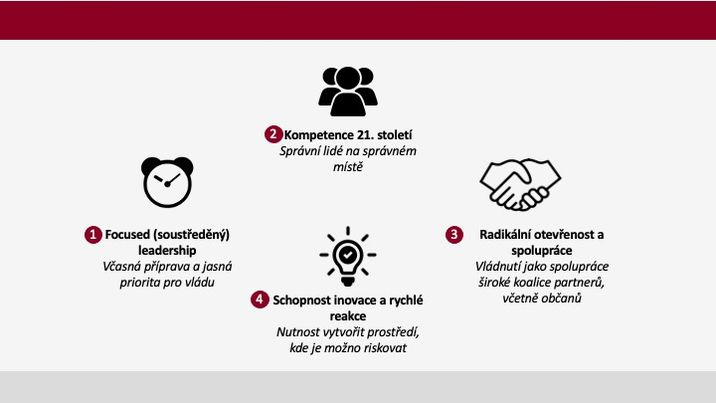
\includegraphics[width=0.8\textwidth]{pic/evaschema.jpg}
    \caption{Čtyři hlavní oblasti pro reformu vládnutí.}
    \label{fig:ctyrioblasti}
\end{figure}

\section*{Úvod} 

Pandemie onemocnění covid-19 ukázala nám všem, že se bez dobrého vládnutí neobejdeme. V~roce 2020 a 2021 měla kvalita rozhodování, implementace a komunikace politiků a zaměstnanců veřejné správy přímé a velmi viditelné dopady na počet úmrtí, na ekonomiku i na společenskou atmosféru.

Koronavirus ostře nasvítil obecnější problémy vládnutí, kterých si je stát dlouhodobě vědom. Například strategie \uv{Klientsky orientovaná veřejná správa} schválená vládou na jaře 2020 konstatuje, že „instituce veřejného sektoru postrádají rychlost a přizpůsobivost, aby udržely krok v~rychle se měnícím světě“ \cite{ministerstvo_pro_mistni_rozvoj_cr_ministerstvo_2020}, výroční zpráva NKÚ za rok 2020 též upozorňuje na „chybějící schopnost státu jednat cíleně a systematicky“ \cite{nejvyssi-kontrolni-urad_vyrocni_2020}. Negativně vychází ČR i z~mezinárodních žebříčků v~této oblasti \cite{wef_global_2019}. Přesto zde vidíme naději na změnu. Pandemie covid-19 ukázala, jak důležitý je funkční stát, a tím důrazně připomněla nutnost zásadních reforem vládnutí. Jako každá krize může být covid-19 katalyzátorem změn. Aby ke změně doopravdy došlo, je ale třeba analyzovat, co se stalo a které aspekty vládnutí je nutno do budoucna změnit.

\newpage 

Cílem tohoto textu je použít přípravu a provedení očkování v~ČR jako případovou studii pro fungování státu. Na příkladu očkování chceme ukázat, jak je potřeba změnit systém vládnutí a fungování veřejné správy tak, aby byl připraven nejen na případnou další krizi podobnou pandemii, ale i obecněji na výzvy 21. století. Naším záměrem není hledat viníky, ale nabídnout úvahu nad systémem a jeho zlepšením.


Očkování je totiž příkladem nového typu výzev. Mají čtyři společné charakteristiky: 1) nejistota vývoje, a tedy i řešení, a rychlé změny parametrů (například o~vývoji či dodávkách vakcín), 2) komplexita (očkování vyžaduje spolupráci mnoha partnerů), 3) role občanů (zvyšující se očekávání týkající se efektivní správy věcí veřejných i uživatelské zkušenosti, zároveň s~nutností aktivního zapojení občanů, 4)~přístup k~technologiím a datům, jež dále zvyšují tato očekávání, případně snižují důvěru občanů ve vládu. Tento typ výzev bude čím dál častější -- jde také například o~globální migraci nebo dekarbonizaci. Jak konstatuje OECD, na dnešní výzvy již nelze nahlížet jako na velké „inženýrské“ projekty, je potřeba je pojímat zcela jinak \cite{oecd_public_governance_reviews_skills_2020}.


V~rámci BISOP jsme se očkováním zabývali dlouhodobě od prosince 2020, spolu s~kolegy jsme napsali více než 20 textů na toto téma. Pro tento článek používáme veřejně dostupná data a mediální výstupy. Na základě naší analýzy navrhujeme čtyři hlavní oblasti, na které doporučujeme se zaměřit při reformě vládnutí. V~textu je postupně rozebíráme a uvádíme příklady jak z~ČR, tak ze zahraničí. Jako příklad používáme zejména přípravu očkování ve Velké Británii, která je v~této oblasti pozitivně hodnocena. Jsme si ale vědomy, že situace v~Británii je v~mnohém jiná. Nepokoušíme se tedy o~přímé srovnání, nýbrž o~inspiraci obecnými mechanismy a~typy řešení.

\newpage

Kvůli zaměření na možná zlepšení systému jsou v~textu výrazněji představeny ty aspekty, které se v~procesu přípravy očkování v~ČR nepovedly. Tím však nechceme zpochybnit zásluhy mnoha lidí na různých úrovních veřejné správy a dalších organizací, kteří pracovali na přípravě a provádění očkování s~obrovským nasazením a zasloužili se tak o~mnohé úspěchy. Naším cílem je představit oblasti možného zlepšení, tak abychom byli na další komplexní výzvy jako stát lépe připraveni.

Jsme si také vědomy, že funkční stát vyžaduje jak schopné politické rozhodování (jehož aktérem je vláda a politici), tak efektivní administrativu (zde jsou aktérem zaměstnanci veřejné správy). Námi vybrané oblasti nutných změn jsou nicméně relevantní pro obě skupiny aktérů a obě také používáme v~ukázkách v~textu. 

\section*{Focused (soustředěný) leadership -- včasná příprava a jasné priority}

\paragraph {Definice:} Každý „decision maker“ (politik či úředník) je dnes vystaven přílivu informací a názorů. Je často nucen se rychle vyjadřovat k~mnoha tématům a rozhodovat. Focused („soustředěným“) leadershipem nazýváme takové vládnutí, při kterém nejvyšší vedení státu včas identifikuje a poté efektivně řídí malý počet priorit. Pro tyto prioritní projekty stanoví jasné cíle a zodpovědnosti a přidělí na ně dostatečné personální i finanční prostředky. Vedoucí představitelé státu pak věnují těmto prioritním projektům podstatnou část své energie, času, případně i politického kapitálu.

\paragraph{Očkování:} Covid-19 uvrhl všechny vlády světa do velmi nejisté situace s~mnoha nečekanými a komplexními problémy. Již na jaře 2020 však bylo zjevné, že očkování je třeba považovat za prioritní směr, za jednu z~nejpravděpodobnějších cest k~návratu do normálu. Bylo též jasné, že rychlost bude klíčová -- každý týden zpoždění při nasazení vakcín bude znamenat ztracené životy a miliardy ekonomických ztrát.

\paragraph{Příklad Británie:} Britská vláda podcenila první vlnu pandemie na jaře 2020. Nejvyšší představitelé státu ale včas identifikovali očkování jako důležitý úkol a věnovali mu dostatečnou pozornost i prostředky v~době, kdy bzla veškerá mediální pozornost soustředěna na zvládání tehdejší situace. Vláda ustanovila již 17. dubna 2020 svoji „Vaccine Taskforce“ (dále VTF) s~cílem podpořit co nejrychlejší vývoj vakcín, upravit regulatorní rámec pro klinické studie a připravit plány pro nákup vakcín a očkování obyvatelstva \cite{department_for_business_energy__industrial_strategy_government_2020}. Komise pro vakcinaci a imunizaci (Joint Committee on Vaccination and Immunisation) se sešla již 7. května 2020 k~diskusi nad prioritizací očkování na covid-19. \cite{department_of_health_and_social_care_joint_2020}. Vedoucí VTF (najatá ze soukromého sektoru) reportovala přímo premiérovi, měla k~dispozici 200 zaměstnanců a široký mandát pro spolupráci s~dalšími resorty, veřejnou správou, soukromým i nevládním sektorem. Vedení státu veřejně označilo očkování za prioritu a věnovalo mu velkou část svých proslovů a~politického kapitálu.

\paragraph{Očkování v~ČR:} V~českém prostředí bylo řešení očkování značně pomalejší a bez dostatečné politické pozornosti. První úvahy o~prioritizaci očkování vznikaly v~rámci České vakcinologické společnosti v~létě 2020, avšak bez formální spojitosti na státní strategie. První oficiální čtyřstránková „strategie“ očkování byla publikována 7. září 2020 \cite{mz2021strat}. Na programu jednání vlády se očkování poprvé objevuje až 30. listopadu 2020 \cite{vlada_prijala_2020}. Celostátním koordinátorem očkování byl teprve 8. prosince 2020 jmenován bývalý ředitel SZÚ Zdeněk Blahuta, upřesněná a podrobnější strategie je vydána až 23. prosince 2020. V~ČR nebylo očkování bráno za prioritu. Nebyl vytvořen žádný specifický koordinační orgán pro řešení otázek očkování. Zodpovědnost zůstala na Ministerstvu zdravotnictví ČR, které ale tomuto tématu nevěnovalo dostatečnou pozornost. Například Roman Prymula, ministr zdravotnictví v~říjnu 2020, uvedl, že se ke strategii očkování po měsíc svého řízení resortu „nedostal“, protože jeho prioritou bylo zastavení velkého počtu nakažených \cite{pokorna_startuje_2020}.

Problém vězel také v~nejasných odpovědnostech a procesech. Klíčovou otázkou pro všechny státy byl nákup vakcín. Ten bylo třeba provést v~době nejistoty o~tom, kdy a které vakcíny v~klinických studiích uspějí. ČR se v~červnu 2020 připojila ke společnému nákupu prostřednictvím EU. Rozhodovací mechanismy týkající se nákupu v~rámci EU však nebyly dány jasně a rozhodnutí proběhlo na základě subjektivních názorů spíše než na základě jasných podkladů. ČR objednala 81 \% \cite{houska_cesko_2021} (jiné zdroje uvádějí 65 \%, \cite{koubsky_slozite_2021}) maximálního množství vakcín, které bylo možné objednat v~rámci EU. To se později ukázalo jako nesprávné a ČR do dubna 2021 zaostávala v~tempu očkování za průměrem EU. Podle vyjádření zástupců MZ ČR neexistuje písemný dokument o~tom, proč ČR objednala pouze 2 miliony vakcín Pfizer, protože tento pokyn sdělil ministr příslušnému odboru pouze ústně \cite{pokorna_proc_2021} . Nejasná situace pokračuje dál, ani v~květnu 2021 nebylo zcela jasné, kdo očkování koordinuje \cite{televize_nevime_2021, skoupa_je_2021}.

\paragraph{Širší kontext/závěr:} Příprava očkování tak poukázala na některé dlouhodobější problémy vládnutí v~ČR -- reaktivní spíše než proaktivní přístup \cite{hlidac_statu_nejvetsi_2020}, neschopnost stanovit malý počet jasných priorit \cite{sedlackova_stat_2020} a dlouhodobě nedostatečnou a nezlepšující se kapacitu pro strategickou práci ve státní správě \cite{ministerstvo_pro_mistni_rozvoj_cr_ministerstvo_2020}. Jak ukazují zkušenosti z~jiných zemí, klíčem k~efektivnímu dosahování cílů je soustředění se na malý počet dobře řízených priorit \cite{allas_delivering_2018, department_of_the_prime_minister_and_cabinet_our_2019, european_social_fund_public_2020}.

Reforma vládnutí v~ČR by měla k~dosažení focused (soustředěného) leadershipu
implementovat následující změny:
\begin{description}
  \item[Prioritizace:] Vláda stanoví a poté pravidelně aktualizuje malý počet hlavních priorit
  \item[Plánování:] Pro tyto prioritní projekty nastaví jasné cíle, zodpovědnost, kompetence, prostředky (lidské i finanční), důsledně aplikuje principy projektového řízení
  \item[Leadership:] Prioritním projektům věnuje premiér a další představitelé státu podstatnou část svého času a energie (účastní se rozhodování, koordinace, komunikace interní i externí)
\end{description}

\section*{Radikální otevřenost -- vládnutí jako spolupráce \\ široké koalice partnerů včetně občanů}

\paragraph{Definice:}Pokud je spolupráce důležitá pro standardní problémy, pro komplexní výzvy zmíněné v~úvodu textu je zcela nezbytná. Nejde o~kosmetické změny, nýbrž o~zcela radikální změnu přístupu. Rigidní vertikální organizace a „resortní“ přístup státu jsou neadekvátní pro nejisté, rychle se měnící a technologické výzvy dneška \cite{d_eggers_future_2020}. Zpráva OECD z~roku 2017 konstatuje, že problémy jsou dnes příliš komplexní na to, aby je stát řešil sám, a komentuje rozostření hranic mezi veřejným, soukromým a neziskovým sektorem \cite{oecd_public_governance_reviews_skills_2020}. Klíčovým partnerem pro stát by samozřejmě měl být občan.

\paragraph{Očkování:} Již v~létě 2020 bylo zjevné, že projekt očkování proti covid-19 bude bezprecedentní operací, která bude vyžadovat masivní logistiku a koordinaci úsilí mnoha různých partnerů, včetně podpory a zapojení všech skupin občanů.

\paragraph{Příklad Británie:} V~Británii byla potřeba větší koordinace u~zrodu VTF. Jejím explicitním úkolem bylo propojit stát, akademickou sféru a průmysl. Projekt očkování byl tedy od začátku pojímán jako intenzivní spolupráce široké koalice partnerů -- státní správy, místních samospráv, NHS, Public Health England, armády, nevládních organizací a soukromého sektoru. Britská vláda také – podobně jako v~ostatních oblastech koronavirového řízení – poskytovala již od počátku pravidelná a detailní data jak veřejnosti, tak nezávislým expertům k~analýzám a komentářům. Spolupráce s~akademickou sférou byla také využita v~otázce definice prioritních skupin \cite{department_of_health_and_social_care_joint_2020}. I~jiné země zadaly přípravu matematického modelu optimální prioritizace skupin vlastním institucím, jako je Robert Koch Institut v~Německu \cite{rki_rki_2021}, nebo externistům \cite{dooling_phased_2020}.

Nemenší důraz věnovala VTF občanům. Komunikace s~veřejností byla jednou z~hlavních oblastí její činnosti, včetně cílené a opakující se komunikace týkající se očkování centrálně i prostřednictvím praktických lékařů a informačních kampaní vytvořených specificky pro hůře dosažitelné skupiny britské populace. To vše určitě přispělo k~vysoké proočkovanosti rizikových skupin -- u~seniorů starších 70 let bylo k~12. červnu 2021 první dávkou očkováno 98 \%  \cite{nhs_statistics_2021} oproti 83 \% ve stejné kohortě v~ČR \cite{noauthor_microsoft_2021}. Pouze cca 15 \% britských občanů hodnotilo v~únoru 2021 průběh očkování negativně \cite{skinner_strong_2021}.

\paragraph{Očkování v~ČR:} V~ČR přistoupilo MZ k~očkování převážně jako k~„resortnímu“ problému. Pozdní zapojení a špatná komunikace s~klíčovými partnery (kraje, praktičtí lékaři) vedly k~neefektivitě (zejména ke zpoždění vakcinace prioritních skupin) i k~pocitu nespravedlnosti (menší dostupnost vakcín v~některých krajích, \uv{předbíhání}, například u~zaměstnanců Státního zdravotního ústavu).

Hejtmani kritizovali především fakt, že informace přicházely pozdě a v~nedostatečné kvalitě \cite{dragoun_hejtmani_2021}. Podobně si na špatnou komunikaci stěžovali i praktičtí lékaři \cite{televize_nevime_2021, prima_delate_2021}. K~intenzivní spolupráci s~nevládním sektorem, zejména s~organizacemi pro seniory, docházelo na úrovni krajů či obcí. Tzv. „community engagement“ (zapojení občanů a komunit do všech fází realizace) ale nebylo součástí celostátní strategie.

MZ periodicky konzultovalo svůj postup i s~externími skupinami (příprava PES, MeSES apod.), i když komunikace byla často problematická \cite{irozhlas_smejkalovu_2021, jerabkova_smejkal_2021}. Spolupráce se po určité době podařila s~iniciativou Cesta ven při přípravě komunikační kampaně \cite{mudrochova_kampan_2020}. Stejně tak úspěšné Národní očkovací centrum v~O2 aréně je výsledkem kooperace několika partnerů (ÚVN, NAKIT -- Národní agentura pro komunikační a informační technologie, Lékaři pomáhají Česku, AČR), včetně pronájmu od soukromého majitele objektu. Mnohé projekty „koalice partnerů“ vznikly na úrovni krajů a obcí. MZ ale nedalo velkou roli akademickému sektoru: Matematický model očkování MZ ČR nevytvořilo ani nikomu nezadalo. Česká prioritizace \cite{strategie_ockovani_mzcr_2020} tak neobsahuje žádný náznak spolupráce s~akademickou sférou nebo „evidence-based“ rozhodování. Stejně tak pokus o~spolupráci s~akademickou sférou v~oblasti vývoje vakcíny strádal nejasnou komunikací s~partnery i vůči veřejnosti \cite{bezdekova_ceska_2021}.

Co se týče \uv{partnerství} s~občany, komunikace o~očkování byla opožděná, málo transparentní a vytvářela chaotický dojem -- prioritizace skupin se několikrát měnila bez dostatečného vysvětlení. V~dubnu 2021 hodnotila průběh očkování negativně více než polovina dotazovaných \cite{cvvm_verejnost_ockovani_2021}. Silně medializovaným příkladem absence orientace na klienta bylo spuštění Centrálního rezervačního systému (CRS) 15.~ledna 2021. Občané očekávali službu srovnatelnou se soukromým sektorem, zatímco nabídnuté řešení nesplňovalo základní parametry jednoduchosti a u\-ži\-va\-tel\-ské\-ho komfortu \cite{blaha_registrace_2021} a nezohlednilo fakt, že jeho první cílovou skupinou jsou senioři. Pandemie obecně obnažila zaostávání ČR v oblasti digitalizace \cite{usela_pres_2021} i absenci pokroku v~této oblasti. \cite{european_comission_desi_2020, hlidac_nedigitalni_2021}.

\paragraph{Širší kontext/závěr:} Příprava očkování na jednu stranu potvrdila, že obecně \uv{vláda i státní správa sází na ,resortismus' -- úzký pohled lidí z~jednoho oboru, a ustálené struktury státní správy}. \cite{hudema_hudema_2021}. Na druhou stranu též ukázala schopnost pracovat v~koalici partnerů, pokud se o~to státní správa pokusí, ať už se to týkalo komunikační kampaně, Národního očkovacího centra nebo projektů na úrovni krajů a obcí.

Jsme přesvědčeny, že nové výzvy by měly vyžadovat právě takovýto partnerský přístup \cite{christopher_blueprint_2021} a reforma vládnutí by v~sobě měla zahrnovat následující aspekty:

\begin{description}
  \item[Otevřenost:] Transformovat veřejnou správu a její pojetí projektů k~skutečnému partnerství s~jinými organizacemi a zbytkem společnosti (samosprávy, akademická sféra, soukromý sektor, média, nevládní organizace atd.).
  \item[Partnerství:] Místo direktivního \uv{řízení} pojímat vládnutí jako \uv{spolupráci široké koalice partnerů} \cite{department_of_the_prime_minister_and_cabinet_our_2019}.
  \item[Spolupráce:] Odstoupit od vertikálního modelu vedoucího k~\uv{resortismu}.
  \item[Orientace na občana:] Koncepci „Klientsky orientovaná veřejná správa“, schvá\-le\-nou v~roce 2020 \cite{koncepce_verejna_sprava_2030} uvést z~teorie do praxe nejen v~otázkách digitalizace.
\end{description}

\section*{Schopnost inovace a rychlé reakce -- nutnost vytvořit prostředí, kde je možné riskovat}

\paragraph{Definice:} Veřejná správa budoucnosti potřebuje schopnost inovovat a rychle reagovat. ČR si důležitost inovací uvědomuje: v~roce 2019 ČR podepsala deklaraci OECD o~nutnosti inovací ve veřejné správě \cite{oecd_deklarace_2019}. Strategický dokument Česko 2030 konstatuje, že „inovace – nejen procesní (administrativní, technologické), ale také inovace ve službách, stylu řízení a inovace konceptuální – jsou bez nadsázky alfou a omegou dlouhodobě udržitelného vládnutí \cite{sr2030}.

Toho je možno dosáhnout změnou v~oblasti systémů a procesů, vytvořením kultury, ve které je možné riskovat, a otevřenou komunikací a nastavením očekávání v~celém ekosystému (NKÚ, média, veřejnost).

\paragraph{Očkování:} Očkování bylo se svými rychle se měnícími a často těžko před\-ví\-da\-tel\-ný\-mi parametry typickým pří\-kla\-dem problému, kdy je třeba experimentovat, pracovat s~upravitelnými scénáři a průběžně se učit z~chyb. Zejména nákup vakcín byl příkladem velmi riskantního projektu s~potenciálně velkým pozitivním dopadem.

\paragraph{Příklad Británie:} V~Británii lze najít příklady, kdy se stát poučil ze svých chyb -- „fiasko“ nákupu zdravotnického materiálu ze strany MZ na jaře 2020 vedlo k~ustanovení nestandardního prvku Vaccine Task Force \cite{balls_secrets_2021}. V~otázce nákupu vakcín Británie svůj způsob rozhodování průběžně přizpůsobovala situaci -- například vytvořila nový ministerský panel, který mohl rychle schválit investice větší než 150 milionů GBP. Došlo také ke zrychlení schvalování -- z~obvyklých čtyř týdnů na 7--9 dnů \cite{national_audit_office_investigation_2020}. Vedoucí VTF Binghamová nedostala „bianco šek“, rozhodnutí probíhalo na základě „business case“ pro jednotlivé vakcíny. Kritéria však byla jasná -- rychlost a efektivita vakcín byla důležitější než náklady na ně \cite{bolzen_kate_2021}. Hlavní představitelé také pravidelně informovali veřejnost o~nejnovějších rozhodnutích a jejich odůvodnění \cite{davis_uk_2020}.

\paragraph{Očkování v~ČR:} V~České republice byl způsob fungování MZ na jaře 2020 (při nákupech OPP, řízení KHS, testování a trasování) svého druhu pilotem řešení nové situace. Navzdory problémům, které se v~této oblasti na jaře 2020 objevily, vláda svěřila projekt očkování opět MZ s~minimální známkou ponaučení se z~jarních událostí.

Na prvotní nesnáze spojené s~neustále se měnícím počtem dodávaných vakcín vláda paradoxně reagovala rezignací na plánování -- vyjádření představitelů vlády na toto téma byla velmi nejasná a nepřesná (například protiřečící si výroky ministra Blatného a MZ týkající se pozastavení prvních dávek či nejasné a měnící se cíle očkování, viz kapitolu \ref{Logistika_ockovani}. Ochotu experimentovat s~inovativními řešeními jsme zaznamenali na nižších úrovních, v~krajích a obcích. Příkladem může být „pilot“ očkování seniorů v~Praze 7, kde se ve dnech 14.--18. ledna 2021 podařilo očkovat 1100 seniorů nad 80 let. \cite{bisop_osloveni_2021}.

Největší dopad mělo rozhodnutí o~nákupech méně vakcín, než činil průměr EU. V~rozhovorech to představitelé státu vysvětlovali tím, že by museli „obhájit utracení velkého množství peněz“ \cite{pokorna_proc_2021}, nebo by prý byli obviněni, že „vyplýtvali peníze daňových poplatníků“ \cite{hronova_kdybychom_2021}.

Takové chování je zcela pochopitelné v~současném systému. Za úspěch při inovaci (např. riskantní nákup vakcín) je možné dostat drobnou odměnu (finanční či nefinanční), zatímco za neúspěšnou inovaci bude úředník podroben kritice ze strany nadřízených, NKÚ, médií i nevládních organizací. Tím se situace liší od soukromého sektoru, kde úspěšné inovace potenciálně vedou k~velkým odměnám.

Tento opatrný přístup byl zjevný během roku 2020 a 2021 -- například při nákupu zdravotnického materiálu na jaře 2020 při první vlně covid-19 \cite{nejvyssi_kontrolni_urad_stat_2021}. V~politické a mediální zkratce je složité rozlišit „chybu, která by se neměla nikdy stát“ (jejímž důvodem je korupce, nekompetence nebo nedostatečné zvážení okolností), a „experimentální chybu“ (jejímž důvodem je pokus o~nejlepší možné řešení v~nejisté či časově napjaté situaci). Pokud žádáme od státní správy schopnost přijmout riziko, je potřeba, aby celý ekosystém (NKÚ, politici, média, veřejnost atd.) chápal komplexnost problému -- nelze nakupovat zdravotnický materiál velmi rychle a přitom zcela bezchybně, je potřeba si vybrat \cite{noauthor_how_2020}.

\paragraph{Širší kontext/závěr:} Příprava očkování nasvítila dlouhodobě zanedbávanou oblast inovací a schopnosti přijímat riziko ve státní správě ČR. V~roce 2017 shrnoval situaci oficiální dokument MV: „Problém je ještě zesilován trvalým mediálně-politickým tlakem, jemuž je veřejná správa jako celek vystavena, a nižší mírou důvěry, kterou v~ní veřejnost má, v~kombinaci s~čím dál detailnějšími definicemi procesních postupů, jež provázejí některé jinak záslužné záměry. Logickým řešením je pak z~hlediska zaměstnanců veřejné správy únik do formalismu a snaha zbavit se v~maximální míře odpovědnosti za jakékoli řešení \cite{pg:polasek2016}. Po třech letech je hodnocení posunu mírně optimistické: \uv{O rozvinutí systému podpory inovací, neřkuli o~změně prostředí zatím nelze mluvit, inovace jsou stále izolovanou a obtížně vybojovávanou aktivitou. Došlo však ke změně atmosféry a prvním reálným krokům, které by mohly vést k~výraznějšímu posunu v~letech 2021–2023} \cite{ministerstvo_pro_mistni_rozvoj_cr_ministerstvo_2020}.

Vzhledem k~novým výzvám, které před námi stojí, bude klíčové tuto oblast
podpořit ve spolupráci celého ekosystému, včetně vzdělávání politiků a
veřejnosti na toto téma.

Možná reforma by tedy měla obsahovat následující komponenty:

\begin{description}
  \item[Systémy a procesy:] Nastavení jasných mechanismů v~případě možné „chyby“, využití agilní metodologie \cite{christopher_blueprint_2021} či inovačních laboratoří ve vhodných oblastech veřejné správy \cite{ministerstvo_pro_mistni_rozvoj_cr_ministerstvo_2020}.
  \item[Kultura:] Změna organizační kultury ve veřejné správě a vytvoření prostředí, kde je možné riskovat a dělat \uv{chyby}.
  \item[Komunikace a očekávání:] Otevřená komunikace s~celým ekosystémem (NKÚ, média, politici, veřejnost, nevládní organizace) o~vhodné míře rizika a jejich důvodech.
\end{description}

\newpage

\section*{Kompetence pro 21. století -- správní lidé \\ na správném místě}

\paragraph{Definice:} Před sto lety bylo možné pohlížet na zaměstnance jako na snadno za\-mě\-ni\-tel\-né součástky. V~dnešním světě jsou ale kvalita a vhodné kompetence lidí zcela klíčové. Úspěšné firmy důraz na práci s~„lidským kapitálem“ v~posledních desetiletích integrovaly do jádra svého fungování. V~této oblasti je také možné pozorovat největší rozdíl mezi soukromým a veřejným sektorem \cite{d_eggers_future_2020}.

Jakákoliv reforma vládnutí by měla zahrnovat důraz na investici do kompetencí pro 21. století, tedy zdánlivě jednoduše \uv{mít správné lidi na správném místě}. Je potřeba plánovat budoucí potřeby s~vědomím změn, které nás čekají. Je také nutné přilákat do politiky i veřejné správy schopné zaměstnance, pracovat na jejich rozvoji, motivaci a správném využití. V~návaznosti na výše popsanou nutnost větší otevřenosti je také záhodné podpořit flexibilnější modely a propustnost veřejné správy a zbytku společnosti.

\paragraph{Očkování:} Příprava očkování dobře ukazuje, že nároky na zaměstnance veřejné správy jsou vyšší než kdykoliv dříve -- pro úspěch byly potřeba technické dovednosti (IT, projektový management atd.), ale také schopnost spolupracovat s~různorodými partnery a rychle se přizpůsobovat situaci. 

\paragraph{Příklad Británie:} Británie přistoupila k~práci s~lidmi v~případě očkování velmi flexibilně. Jedním z~důvodů pro vznik Vaccine Task Force (VTF) byla právě obava, že v~britské státní správě neexistuje dostatečná expertíza o~vakcínách \cite{balls_secrets_2021}. Do čela VTF byla v~polovině května 2020 jmenována Kate Binghamová \cite{department_for_business_energy__industrial_strategy_statement_2020}, zkušená investorka do~bio-tech\-no\-lo\-gií, pro své \uv{vyjednávací schopnosti a globální reputaci} \cite{department_for_business_energy__industrial_strategy_statement_2020}. Její funkce byla neplacená a omezená na 6~měsíců. V~listopadu 2020 měla VTF 200 členů, 120 bylo přesunuto z~jiných pozic ve státní správě (celkově došlo v~Británii mezi březnem 2020 a březnem 2021 k~přesunutí více než 3000 úředníků do kritických rolí spojených s~řešením pandemie). Zbylých 80 pracovníků VTF bylo najato ze soukromého sektoru. Ve vedení VTF tak bok po boku pracoval například expert se zkušenostmi jako generální ředitel farmaceutické společnosti se specialistou na nákup z~armády \cite{national_audit_office_investigation_2020}.

\paragraph{Očkování v~ČR:} Ve veřejné správě v~ČR pracuje mnoho schopných a motivovaných zaměstnanců. Přesto si jenom 16 \% občanů myslí, že \uv{ve státní správě pracují ti nejschopnější}, a pouze 23 \%, že \uv{státní správa má dobrou pověst} \cite{aspen_vnimani_2021}.

Očkování bylo jen jednou z~oblastí, která odhalila nedostatky na Ministerstvu zdravotnictví a některých jemu podřízených organizacích -- nedostatečný personál na pokrytí vybrané agendy a chybějící expertíza. Na rozdíl od mnoha jiných evropských států, česká státní správa kromě několika výjimek (zejména prostřednictvím NAKIT a za využití Armády ČR) nenabírala nové pracovníky či přímo týmy pracovníků na pokrytí nutných prioritních projektů.

Jestli je již dnes složité najít pracovníky s~odpovídajícími kompetencemi, nároky budou v~příštích desetiletích stoupat. Jedná se o~tři typy dovedností:
\begin{description}
  \item[Technické kompetence] -- například IT, datové
analýzy, projektové řízení \cite{thomas_finding_2021, hlidac_nedigitalni_2021}.
  \item[„Měkké“ kompetence] -- například schopnost inovace, spolupráce
s~různorodými partnery, rozvoj lidí \cite{oecd_public_governance_reviews_skills_2020}.
  \item[„Metakompetence“] -- například schopnost se učit, řídit změnu, mentální flexibilita \cite{dondi_future-citizen_2020}.
\end{description}
Řízení lidských zdrojů ve státní správě je pojímáno především z~právního a administrativního pohledu. V~tomto směru je pozitivní, že náměstek MV pro státní službu Petr Hůrka \cite{plihalova_z_2020} hovoří o~potřebě zlidštění, zcivilnění a větší flexibilitě jako o~předpokladu zvýšení atraktivity státní správy pro mladé \cite{mpo2021}. Kromě legislativních změn je ale potřeba strategicky plánovat.

Po vzoru jiných zemí \cite{thomas_finding_2021, ministere_gestion_2015} je vhodné porovnat budoucí potřeby se současným stavem a naplánovat, jak případné mezery překlenout. Zmapování současných dovedností by též umožnilo větší flexibilitu zapojení úředníků -- tedy „vypůjčování“ odborníků na jiný projekt či resort. Některé činnosti bude potřeba navíc koncipovat zcela jinak -- odborníci se shodují, že 25--40 \% času tráví úředníci úkoly, které by bylo možné jednoduše automatizovat \cite{department_of_the_prime_minister_and_cabinet_our_2019, deloitte_augmented_2017}. Zajímavým příkladem dopadů technologických změn byly během pandemie proměny trasování, viz kapitolu \ref{Trasovani}.

Paralelně se strategickým plánováním lidského kapitálu ve státní správě je po\-tře\-ba změnit mnohé procesy a posunout tak flexibilitu státní správy blíže k~soukromému sektoru.

Větší mobilita může být dosažena vytvořením „flexibilních“ týmů se všeobecnými dovednostmi, například jako britská Priority Projects Unit, které jsou pak nasazovány do oblastí s~největší momentální prioritou a potřebou kapacit. ČR těchto prvků využívala sporadicky, ale úspěšně. Příkladem je tým „Chytré karantény“ (Centrální řídící tým), který působí od jara 2020 a kombinuje příslušníky AČR a pracovníky NAKIT. Specifické postavení NAKIT (státní podnik) mu umožňuje jednodušeji najmout odborníky na krátkodobý úvazek.

Jednou z~praktických změn může být posun při náboru zaměstnanců. Pro zcela nestandardní a klíčovou roli ředitele pro komunikaci MZ v~lednu 2021 byly využity standardní postupy včetně navrženého platu \cite{irozhlas_ministerstvo_2021}. Je nutné též změnit způsoby kompenzace pro standardní i nestandardní úkoly -- například odměna pro krajské koordinátory očkování v~hodnotě 300 Kč/hodinu byla neadekvátní této klíčové roli \cite{michal_blaha_pandemie_2021}.

\paragraph{Širší kontext/závěr:} Bez schopných lidí s~adekvátními kompetencemi nebude možné uspět ani v~jiných aspektech změny zmíněných v~textu. Veřejná správa potřebuje dohnat soukromý sektor a modernizovat svůj způsob práce s~lidskými zdroji.

Mezi hlavní prvky změny práce s~lidskými zdroji patří:

\begin{itemize}
  \item Systematicky plánovat budoucí potřeby lidského kapitálu s~vědomím nutných změn (automatizace, nové technické i „měkké“ kompetence).
  \item Nastavit flexibilnější modely pro využití existujících pracovníků či krátkodobé najímání expertů.
  \item Zlepšit způsob náboru zaměstnanců -- například nastavit flexibilnější kompenzaci navázanou na výkon, umožnit flexibilní formy práce (home office, částečný úvazek), rozvinout možnosti kariérního růstu a vzdělávání a učinit manažery na všech úrovních zodpovědné za rozvoj členů jejich týmů \cite{thomas_finding_2021, mckinsey_desetileti_2021}.
  \item  Zvýšit atraktivitu práce ve veřejné správě (zejména pro experty a mladé absolventy) -- veřejná správa může využít motivaci pomocí smysluplné práce, která je pro uchazeče o~zaměstnání čím dál tím důležitější (\cite{achor_9_2018} a přilákat nadějné absolventy pomocí speciálních programů běžných v~jiných zemích \cite{noauthor_home_2020, mckinsey_desetileti_2021}.
\end{itemize}

\section*{Diskuse}

V~tomto textu jsme si daly za cíl využít přípravu a provedení očkování jako pří\-pa\-do\-vou studii pro návrh nutných širších změn ve veřejné správě.

Čtyři oblasti, které jsme identifikovaly, považujeme za klíčové. Samozřejmě jsou také navzájem propojené -- například větší propustnost mezi soukromým, akademickým a veřejným sektorem je důležitá jak obecně, tak v~případě práce s~lidmi a~bude mít dopad i na schopnost inovací.

Přály bychom si, aby byl covid určitým „budíčkem“ ke změnám. To se ale může stát jen, pokud jsme schopni situaci analyzovat a poučit se z~ní. Doufáme, že k~analýze podobné (a přesahující) tu naši dojde na úrovni státu nejenom v~otázce očkování. Rády se takového dialogu zúčastníme.

Omezením naší studie je práce pouze s~veřejnými zdroji. Dalším směrem zkoumání by mohly být kvalitativní rozhovory s~hlavními aktéry a pochopení, jak situaci vnímali oni sami. Dalším omezením, daným rozsahem článku, je zaměření se na centrální úroveň řízení. Naše spolupráce s~hlavním městem Praha na přípravě strategie očkování \cite{hygienicka_stanice_praha_2021} svědčí o~tom, že situace na nižších úrovních je v~mnoha ohledech rozdílná. Bylo by zajímavé prozkoumat přípravu očkování právě na úrovni krajů a obcí. Posledním omezením, které jsme již zmínily v~úvodu, je soustředění se na nedostatky spíše než na úspěchy. Dalším směrem zkoumání by mohlo být analogické „ponaučení“, které by stavělo na pozitivních příkladech na všech úrovních. Ambiciózním projektem by pak bylo provést systematické srovnání přípravy očkování ve více zemích, včetně objektivních kritérií úspěchu (proočkovanost rizikových skupin, rychlost očkování atd.).

\section*{Poděkování}

Rády bychom poděkovaly za cenné podněty a konzultace kolegům z~BISOP.
Za příležitost podílet se na přípravě očkování pro hlavní město děkujeme pražské radní pro oblast sociální politiky a zdravotnictví Mileně Johnové.


